\chapter{Experimental results}
\label{chap:results}


\section{Anomaly detection performance}
\label{sec:performance}

With parameters learned from \Fref{sec:parametertuning}, autoencoders are trained for each dataset with the beginning of streaming data. The anomaly detection performance is indicated by AUC. For each dataset, we compare the AUC of online phase that without and with continuously model and parameter updating (\Fref{tab:performance}). For the PowerDemand dataset, retrain trigger depends on the batch performance. And for the rest datasets, retraining only triggered when retrain buffers are full. The retraining brings overall performance improvement on all datasets comparing to stationary models. Especially in the SMTP+HTTP dataset, the stationary without learning concept drifted knowledge performs clearly worth than the model with updating.\\

\begin{table}[h] 
\caption{Performance} 
\centering      
\begin{tabular}{c | c | c | c}  
\hline  
Dataset & AUC(without retraining) & AUC(with retraining) & \#retrain \\ 
\hline 
PowerDemand & 0.91 & 0.97 & 2  \\  
\hline 
SMTP & 0.94 &  0.98 &  2 \\ 
\hline 
HTTP & 0.76 &  0.86 &  2 \\ 
\hline
SMTP+HTTP & 0.64 & 0.85 & 3 \\
\hline 
ForestCover &0.74&0.82 & 8\\   
\hline    
\end{tabular}
\label{tab:performance}  
\end{table} 
In order to compare the performance with and without retraining, after each model updating, we calculate the AUC value for each specified time period. As Shown in \Fref{fig:auc_retrain}, the x-axis represents the periods, for example, before first retraining(shown as P1 in each subplot), between first and second retraining (P2), and so on. For each dataset, we compare the AUC value of stationary model (trained with only initialization set) and adaptive model (online updated). For most cases, the adaptive models outperform stationary models, which shows the models profits from the knowledge updating over streaming data. To be notice that the SMTP+HTTP set contains sudden concept drift around P3, which leads to a sharp decline of the stationary model. In the meantime, the adaptive model is only slightly influenced by the mixed knowledge at P3 but keeps outstanding performance when the stream switches to HTTP side.\\
\begin{figure}[h]
\centering
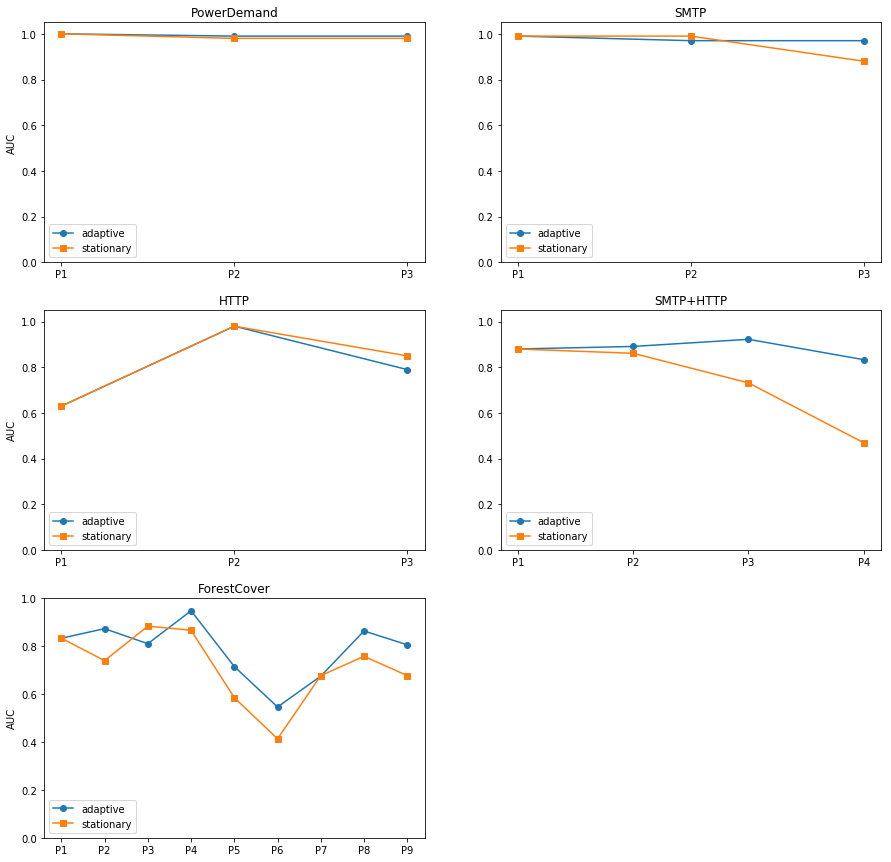
\includegraphics[width=15cm, height=15cm]{auc_retrain}
\caption[AUC comparation between stationary and adaptive models over stream]{AUC comparation between stationary and adaptive models over stream. The x-axis represents specific periods over stream. For example, P1 is the period from beginning to the first retraining, and P2 is the the period between first and second retraining etc.}
\label{fig:auc_retrain}
\end{figure}

\Fref{fig:runtime} shows the run time used for both stationary models and adaptive models for each data set. The updating takes more time for HTTP, SMTP+HTTP and ForesrCover than PowerDemand and SMTP is due to that larger datasets take more time for prediction, and trigger more updating events. And for each retraining, the retrain buffers also contain larger retraining sets.\\



\begin{figure}[h]
\centering
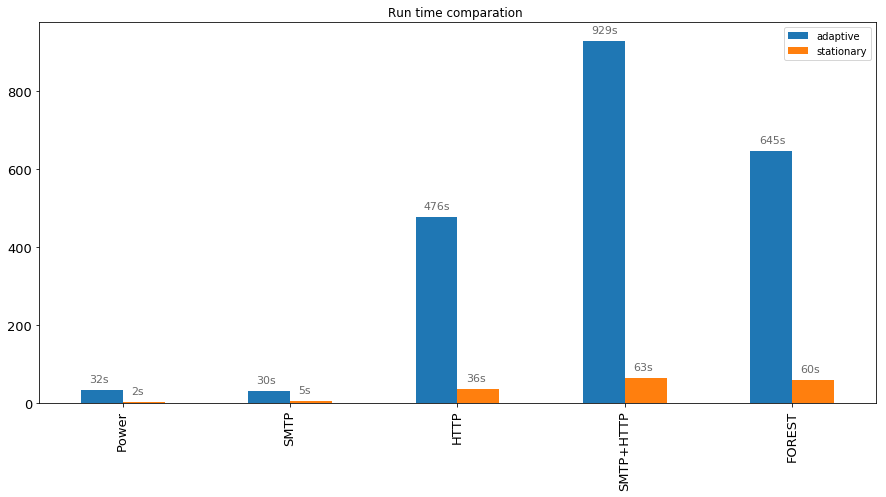
\includegraphics[width=15cm, height=7cm]{runtime}
\caption[Run time statistics]{Run time statistics}
\label{fig:runtime}
\end{figure}


\section{Synthetic example}
\label{sec:synthetic}

In order to show the benefit of model updating over the stream, we demonstrate the online learning process of the small set PowerDemand in this section. The PowerDemand dataset does not contain clear incremental or sudden concept drift, but the normal patterns still different slightly to each other. The lack of overall impression during the model initialization phase can lead to failures during the online phase. \\

\subsection{Anomaly detection over stream}
\label{sec:detection}

Generally, the autoencoder reconstructs normal data with relative lower reconstruction error while anomaly data with significant larger reconstruction error. \Fref{fig:power_re} demonstrates two typical data windows (weeks) in PowerDemand, one normal and one anomaly. The Monday of anomaly week (right) is a special data, which has an abnormally low power demand. Even so, the autoencoder still reconstructs the Monday as usual with a higher score, therefore the reconstruction error is obviously larger on Monday, and the model labels this week as anomaly.\\

\begin{figure}[h]
\centering
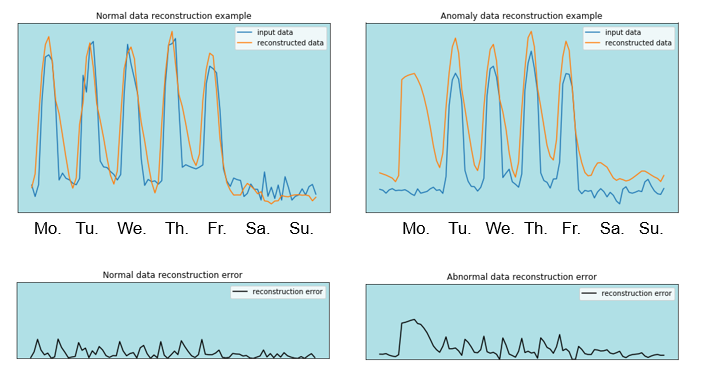
\includegraphics[width=12cm, height=8cm]{power_na}
\caption[Reconstruction error of PowerDemand data]{Reconstruction error of PowerDemand data}
\label{fig:power_re}
\end{figure}

Even there will be concept drift over the stream, which will lead to an entirely increase or decrease in the input side, and the decoder output side remaining, our model can still deal with this problem with its online parameter updating ability. While the anomaly scores are calculated by the mahalanobis distance to the estimated normal distribution of normal data reconstruction errors in the validation set, by every model updating, the model estimates new normal distribution and relevant parameters with the latest collected validation set, so that the reconstruction error based anomaly detection is robust against concept drift.\\



\subsection{Reaction of concept drift}
\label{sec:reaction}

\Fref{fig:power_retraining} shows 3 continual days power demand in normal state. Due to the lack of knowledge for current pattern, the autoencoder reconstructs the input time series higher than desired on day 1 (left diagram). This could be caused by seasonal changes on the power demand, which is slightly, gradually, and would potentially cause misclassification. The increase of normal data reconstruction error makes the margin between two classification classes smaller, and harder to make decision. As a consequence, the model retraining process is triggered after the second day with last seen data in the buffers, and the model performs well again on the third day.\\

\begin{figure}[h]
\centering
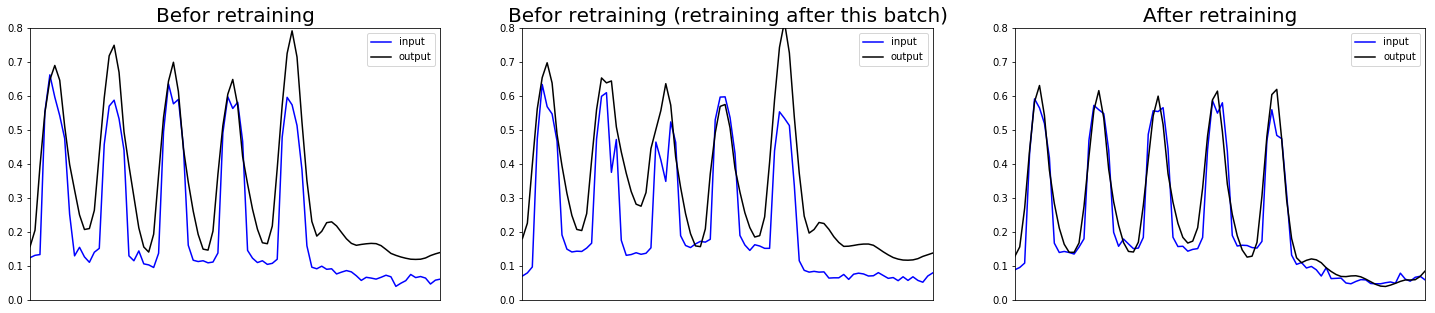
\includegraphics[width=15cm, height=4cm]{power_retraining}
\caption[Retraining effect on PowerDemand dataset]{Retraining effect on PowerDemand dataset}
\label{fig:power_retraining}
\end{figure}

\subsection{Model updating}
\label{sec:retrainig}

During the online phase, the model is retrained two times, before batch No.10 and No. 27. After retraining, the normal data reconstruction error becomes lower while for abnormal data becomes higher, so that the classification becomes easier.\\

\begin{figure}[h]
\centering
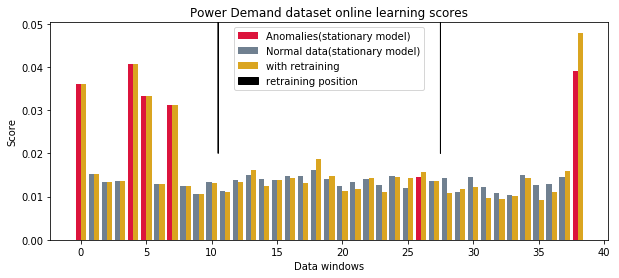
\includegraphics[width=10cm, height=4cm]{power_online_score}
\caption[PowerDemand dataset online learning scores]{PowerDemand dataset online learning scores. For each window, the anomaly score is the highest pointwise scores within the window}
\label{fig:power_online}
\end{figure}

After each updating process, the parameters mu, sigma and threshold of anomaly scores are also updated. \Fref{fig:parachanges} shows the parameter changes over the stream. As there is no clear concept drift during the power demand stream, the parameters change just slightly in oder to learn latest knowledge from the retrain buffer. \\

\begin{figure}[h]
\centering
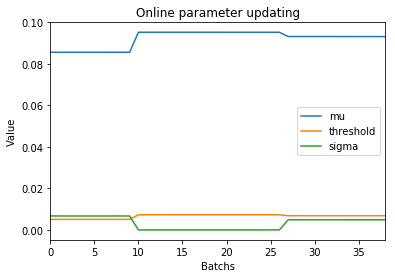
\includegraphics[width=6cm, height=4cm]{para_update}
\caption[PowerDemand dataset online parameter updating]{PowerDemand dataset online parameter updating}
\label{fig:parachanges}
\end{figure}



\section{Model retraining}
\label{sec:retraining}

\subsection{Reaction of sudden and drastic concept drift}
\label{sec:reaction}

The main advantage of online model is its ability to take reaction against sudden data distributional changes over time. The SMTP+HTTP data set is composed by directly connecting HTTP set after SMTP, so there is a sudden concept drift in between. The model is initialized with only SMTP data, so HTTP is completely unknown knowledge for the model. \Fref{fig:smtp+http} shows the scores for both normal and abnormal data over the SMTP+HTTP stream. In the beginning, only SMTP data in the stream, and partially used for model initialization. In the online prediction phase, once the HTTP data arrives, the first peak of normal data scores’ curve appears, and then the model updating is triggered, with buffer data being few hard SMTP data and most HTTP data. After the first model updating, the performance of model is still suboptimal due to the lack of enough HTTP data, therefore there are two further model updating process triggered during the following stream. As a result, the overall anomaly detection for SMTP+HTTP stream is good only except the short period after concept drift. The model updating are triggered in time after concept drift, and afterwards no redundant updating are triggered.\\

\begin{figure}[h]
\centering
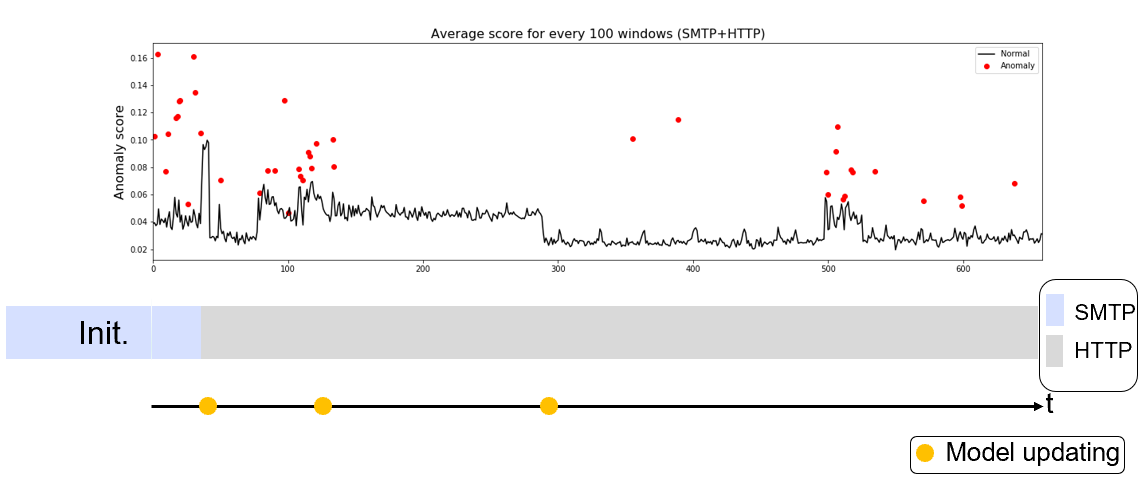
\includegraphics[width=15cm, height=7cm]{sh_conceptdrift}
\caption[SMTP+HTTP stream concept drift]{SMTP+HTTP stream concept drift.}
\label{fig:smtp+http}
\end{figure}

\subsection{Reaction of serial concept drift}
\label{sec:reaction}

Sometimes concept drift over the stream are slight, periodically, and potentially repeated. A single slight concept drift may not be able to trigger the retraining, but new knowledge should be saved into retraining buffer, so that once the model retrained with the fresh knowledge, tshe model should perform well when the same concept drift happens. We experiment with the ForestCover dataset. There are 7 kinds of forest cover types as labels. We take the least TYPE4 as anomaly while the rest 6 kinds as normal. The ForestCover stream is generated type by type, as shown in the bottom chart of \Fref{fig:fcd}. During the beginning phase, TYPE1 data appears in the stream, part of which is used for model initialization. Afterwards follows instances from TYPE2, TYPE3, TYPE5, TYPE6, TYPE7 and finally TYPE2 appears again during the ending phase. Anomaly data (TYPE4) is randomly distributed in the stream. Because the model is only initialized with TYPE1 data, every appearance of a new cover type will potentially cause a performance decrease. The concept drift under this setting is then the type changes over stream. \\

The points on the time axis in \Fref{fig:fcd} indicates the model updating. In the anomaly score chart, the scores for anomaly data are generally larger than normal data except when concept drifts take place. Once data stream from a new cover type appears in the stream, there are always peaks in the normal data score plot, and the difference to anomaly data scores decreases. After performance being impacted, the normal buffer is filled with hard windows shortly, that triggers the model updating quickly after the concept drift. \\

During the experiment, there are two cases delay the updating. Firstly, because of the fixed size of buffer, if a model updating is just triggered shortly before a concept drift, then the hard windows from new cover type need more time to fill the buffer and trigger updating. In \Fref{fig:fcd}, before TYPE3 arrive, there was a updating at the end of TYPE2, and buffered was emptied, so that the model didn’t take any action against the concept drift. Secondly, if a concept drift only appears in a short period, e.g. the TYPE7, which is also not enough to fill the buffer and trigger updating. However, under both aforementioned cases, the new information of concept drift, namely the new cover types, are stored in the buffer, and will be used for next model updating. If the concept drift missed model updating due to too short appearance period, we suppose that this would also not cause catastrophic effect over the stream prediction.\\

\begin{figure}[h]
\centering
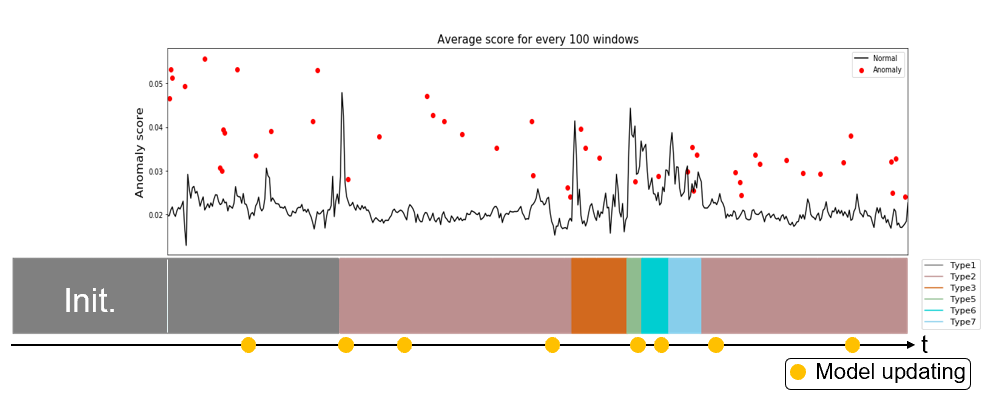
\includegraphics[width=15cm, height=8cm]{forestconceptdrift}
\caption[ForestCover stream concept drift]{ ForestCover stream concept drift. The chart on the bottom shows the cover type over the stream. The top chart shows average anomaly scores for every 100 windows}
\label{fig:fcd}
\end{figure}


\subsection{Summary}
\label{sec:summary}

In this section, we experimented out online LSTMs-Autoencoder model with five different streaming data. With the PowerDemand dataset, we demonstrated a synthetic example of our model, which shows the reconstruction error based anomaly detection mechanism and how the reconstruction adapt to new coming streaming data through model updating. Furthermore, we use the two dataset that contains obvious concept drift, SMTP+HTTP and ForestCover. The model reacts quickly to sudden and drastic concept drift, and potentially more updating will be triggered after concept drift to catch enough valuable information from the drifted stream. And when multiple concept drifts happen temporally and shortly, the model misses some of them, but the fresh information of those concept drifts are still accumulated to the buffer and used by next updating.\\







